\section{Bluetooth in Android}

For the scope of this work, we are specifically interested in the way Bluetooth and Wi-Fi Direct are implemented in Android devices. Various Bluetooth versions have been developed for Android systems. Bluetooth versions over 4.0 are the currently employed in Android devices thus, this study mainly be focused on these versions.

In the following subsections, three use cases of the Bluetooth technology in Android devices will be explained more specifically, how to achieve: a star network, an ad hoc network and multi-hop routing. When appropriate, analysis on previously developed works will be presented, to further demonstrate how these use cases can be achieved using the Bluetooth technology.

\subsection{Bluetooth Star Formation}
\label{subsec:btstar}

In this subsection, the Bluetooth star topology and how it can be achieved in Android systems will be discussed.

As mentioned in Subsection \ref{subsection:bt}, Bluetooth is able to achieve a star network by creating \textit{piconets}, see Figure \ref{fig:bluetooth}. A master node manages the communications with the slaves, by coordinating the medium access of the various devices in the \textit{piconet}.

In Android, depending on the device's hardware, it is possible to establish several concurrent Bluetooth connections between devices - see \cite{btmultipleconn}. A master device is not able to connect to multiple \textit{piconets} and form a \textit{scatternet}, as mentioned in Subsection \ref{subsection:bt}. As mentioned in \cite{btmasterchoice}, the role of a device can not be altered in the user space, see Figure \ref{fig:btstack}, being is defined in the baseband and link controller layer of the Bluetooth chipset. This inability of choosing whether a device acts as a master or slave may impact the \textit{piconet} formation process. In Android, it is common to name the Bluetooth roles of a device, server and client, referring to the device that accepted and requested the connection, respectively. This nomenclature may be misleading, as the server may not be the master and the client may not be the slave.

\begin{figure}[ht]
	\noindent\makebox[\textwidth]
	{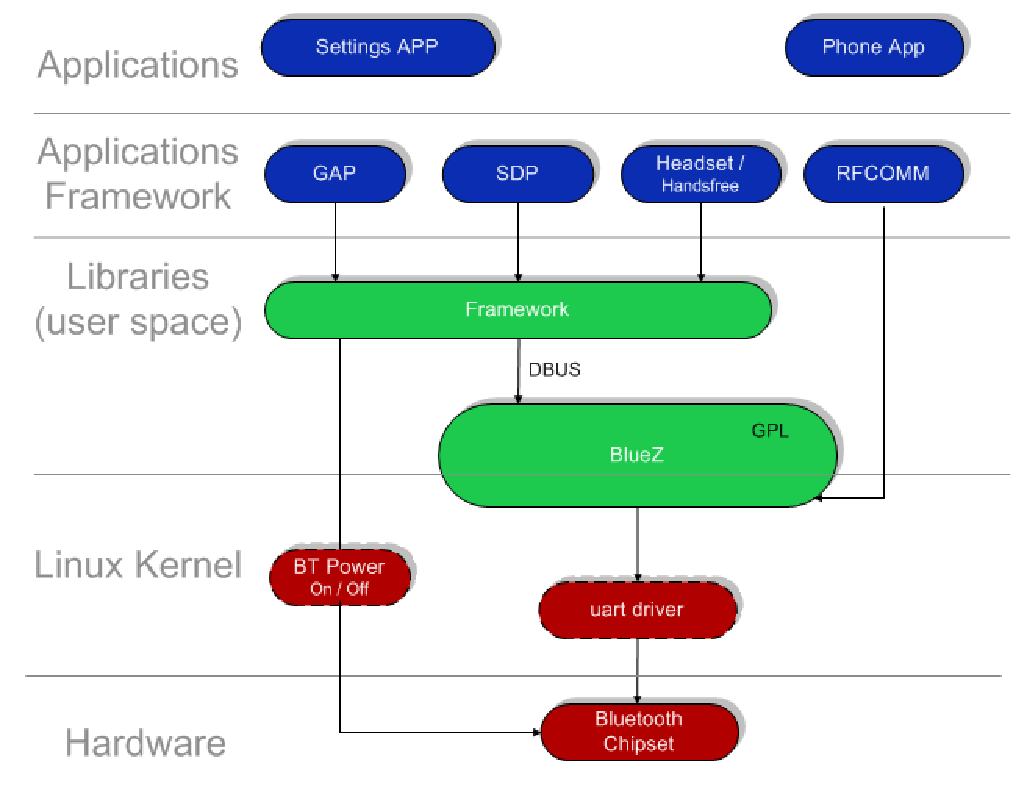
\includegraphics[width=1\textwidth]{images/btstack.pdf}}
	\caption{\label{fig:btstack} Bluetooth protocol stack in Android devices. (source: \cite{androidbtintro})}
\end{figure}

Several applications have been developed, to establish a Bluetooth \textit{piconet} in Android devices\footnote{Two GitHub repositories with Android applications claiming to form a Bluetooth \textit{piconet}: \url{https://github.com/jonnysgomes/piconet/blob/master/src/com/example/piconet/Piconet.java} and \url{https://github.com/ilteoood/bluetooth_piconet/tree/master/app/src}.}. However, these applications assume the device is able to maintain seven active connections which, as mentioned above, depends on the device's Bluetooth hardware.

To create a \textit{piconet}, seven different \glspl{UUID} are created, one for each peer device. The \textit{piconet} establisher device, proceeds to begin a discovery process, where the nearby devices with Bluetooth on will be discovered, \textit{i.e.}, the device that initiated the discovery will have access to the nearby device's Bluetooth name and \gls{MAC} address. Once the device finishes the discovery process, it attempts to establish a connection with each peer device, it is important to note that this device may not be the master, as seen before. For each successful connection attempt, the peer count is increased by one, until a maximum of seven devices is reached. For each connected device, a communication socket is opened, for data transfer between the pair, establishing one, or a \textit{scatternet}, depending on the master/slave role assignment.

\subsection{Ad Hoc Networking}

In the Bluetooth standard, ad hoc networking is achieved through the creation of \textit{piconets} and \textit{scatternets}. As mentioned in the previous subsection, a \textit{piconet} uses a central node, master, and several leaf nodes, slaves, creating an ad hoc network, where the focal point is the master. When several \textit{piconets} are communicating, several master nodes act as focal points of the network, thus creating a decentralized network.

In Android, establishing a \textit{piconet} is challenging, due its lack features, such as the choice of master/slave roles for a specific node. However, some works already approached this problem, see the previous subsection.

In \cite{basa}, D. Zhang \textit{et al.} propose a system architecture to deploy a mobile ad hoc social network in Android systems. They establish four layers to this architecture: device, network, community and application layer. To analyse the formation of an ad hoc network using this architecture, the focus will be in the network layer.

In Figure \ref{fig:basanet}, the authors of \cite{basa}, propose a preliminary network model, based on the proposed scheme. It is possible to see the formation of several \glspl{MANET}, connected by a central sub-network with Internet access, resembling the formation of a \textit{scatternet}. In each \gls{MANET}, mobile devices establish a linear communication topology, meaning that they hold a maximum of two connections, whereas computers may establish meshed networks between themselves and other devices, as seen in the Figure \ref{fig:basanet}.

\begin{figure}[ht]
	\noindent\makebox[\textwidth]
	{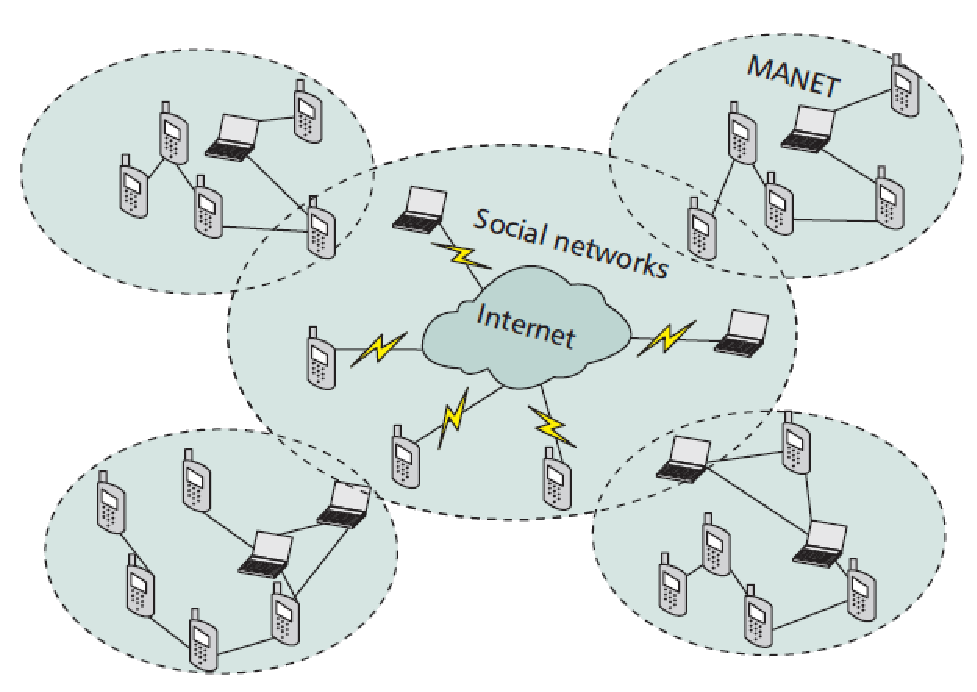
\includegraphics[width=1\textwidth]{images/basanet.pdf}}
	\caption{\label{fig:basanet} Overview of the preliminary network model of the proposed scheme. (source: \cite{basa})}
\end{figure}

It is also stated in \cite{basa} that two distinct problems of the Bluetooth technology in Android systems must be overcome: having no ad hoc function and its constraints of limited power, computation and communication capabilities. The authors state that both these limitations of state of the art Android systems are overcome by the proposed architecture, by (1) allowing devices to discover its neighbouring devices and then, creating local communities, as shown in Figure \ref{fig:basanet}; (2) establishing local networks within smaller areas, where devices are physically close to each other and by developing a lightweight client to server communication protocol.

In \cite{bluehoc}, G. Hinojos \textit{et al.} propose a different approach to create an ad hoc network in Android devices using Bluetooth. To achieve ad hoc networking the authors created what they called \textit{BlueHoc}, a static ad hoc network, composed of a "boss" and several "workers".

In Figure \ref{fig:bluehocnet} an overview of a generic \textit{BlueHoc} network model is shown. The "boss" node may be connected with up to seven "workers", similarly to what happens in a traditional Bluetooth \textit{piconet}. \textit{BlueHoc} networks are static, meaning once a worker connects with a boss it stays connected until the end of the job period.

"Bosses" are able to issue job requests, that are distributed through the "workers". When a "worker" finishes the job, it sends the results back to the "boss" node. With this mechanism, the authors state that it is possible to achieve parallel computation within a \textit{BlueHoc} network.

\begin{figure}[ht]
	\noindent\makebox[\textwidth]
	{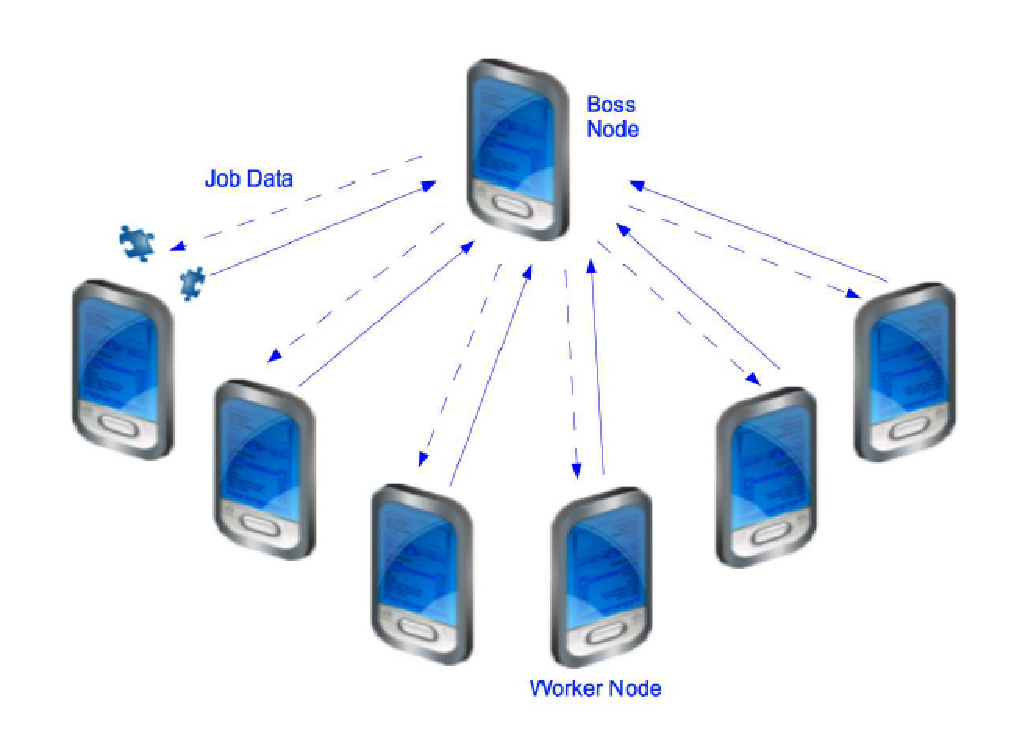
\includegraphics[width=1\textwidth]{images/bluehocnet.pdf}}
	\caption{\label{fig:bluehocnet} Overview of a preliminary network model and data exchange architecture of \textit{BlueHoc}. (source: \cite{bluehoc})}
\end{figure}

In \cite{bluehoc}, G. Hinojos \textit{et al.} point that, future work may lay in the development and implementation of more elaborate protocols, for "scatter-gather-broadcast", substituting the current basic networking architecture.

\subsection{Multi-Hop Routing}

In this subsection, possible approaches to overcome multi-hop routing in Android devices will be presented.

In the previous subsection, the presented works focus on the creation of ad hoc networks. However, none of the described works tackles multi-hop routing. In fact, most of the works are focused on establishing local networks, based on proximity between connected devices. For this thesis, multi-hop routing is a limitation that must be overcome, in order to successfully implement the proposed framework and application - see \ref{sec:objectives}.

Bluetooth in Android, naturally and implements multi-hop. As seen in the previous subsection, mobile devices can connected in a linear network topology, where each mobile device has up to two concurrent connections. However, routing data through these communication links requires additional logic, to ensure the information reaches the correct destination.

In \cite{bwmesh}, Y. Wang \textit{et al.}, propose a multi-hop connectivity framework on Android, using Bluetooth and Wi-Fi Direct as communication technologies, called \textit{BWMesh}. This framework discovers and connects neighbour users, using both Bluetooth and Wi-Fi Direct, transmits messages and provides network status to applications using the framework.

\textit{BWMesh} uses Bluetooth and Wi-Fi Direct's discovery processes to scan for nearby devices. Once two devices are connected, \textit{BWMesh} attempt to maintain their connection as long as possible, for instance by enabling Wi-Fi Direct when a current Bluetooth connection is broken, due to devices being out of Bluetooth communication range.

To communicate between themselves, devices may use Bluetooth or Wi-Fi Direct, depending on the radio interface enabled by the user. However, connection and message transmission may only occur between two Bluetooth or Wi-Fi Direct terminals, not being possible cross-technology communication.

A preliminary simple flooding-based forwarding mechanism is implemented, where a received message is disseminated by the receiver to its nearby peer devices. Also, to unequivocally distinguish devices in a network, the authors proposed a device identifier to be an integration of a user-defined semantic name with the intrinsic device serial number. This identification is technology independent, as both Bluetooth and Wi-Fi have different \gls{MAC} addresses, in an Android device.

In Figure \ref{fig:bwmsg}, the \textit{BWMesh} message formate is shown. The exchanged messages are divided in four segments, each segment being parsed through the corresponding prefix. Prefix (1) \textit{HOP\_NUM} denotes the number of experienced hops transferred from the message originator, each time the message is forwarded a unit is added to this segment; (2) \textit{USER\_NAME} corresponds to the user-defined semantic name, it is used to associate a device with an easily human readable identifier; (3) \textit{DEVICE\_TAG} is the unique identifier of the device in the network; (4) \textit{PAYLOAD\_TXT} is the message content to be transmitted.

\begin{figure}[ht]
	\noindent\makebox[\textwidth]
	{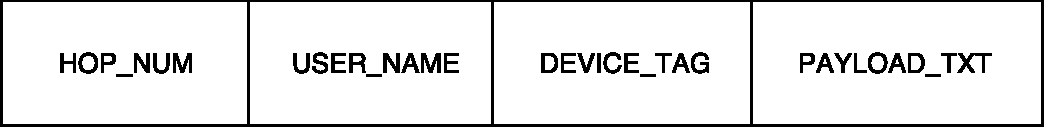
\includegraphics[width=0.8\textwidth]{images/bwmsg.pdf}}
	\caption{\label{fig:bwmsg} \textit{BWMesh} message format.}
\end{figure}

Similarly to what is proposed for this work in Section \ref{sec:objectives}, in \cite{bwmesh} the authors designed and implemented a \textit{BWMesh} based prototype Android application, named \textit{MultiChat}.

\textit{MultiChat} enables users to exchange real-time text messages with nearby people in a multi-hop manner, when they are beyond single-hop Wi-Fi Direct range or without an active Internet connection.

In Figure \ref{fig:bwmeshnet}, a possible network of \textit{MultiChat} is shown. Four users are presented: A, B, C and D. Between A and B, and C and D, a Bluetooth connection is established. Between users B and C a Wi-Fi Direct connection is established.

Once the devices are all connected, as shown in Figure \ref{fig:bwmeshnet}, the four users are able to exchange text messages in a broadcast manner, similarly to a community chat. Also, although user A is not in communication range of user D, they are able to communicate. Using \textit{MultiChat}, every user has knowledge on the unique identifier and number of hops separating him/her from the remaining users of the network.

\begin{figure}[ht]
	\noindent\makebox[\textwidth]
	{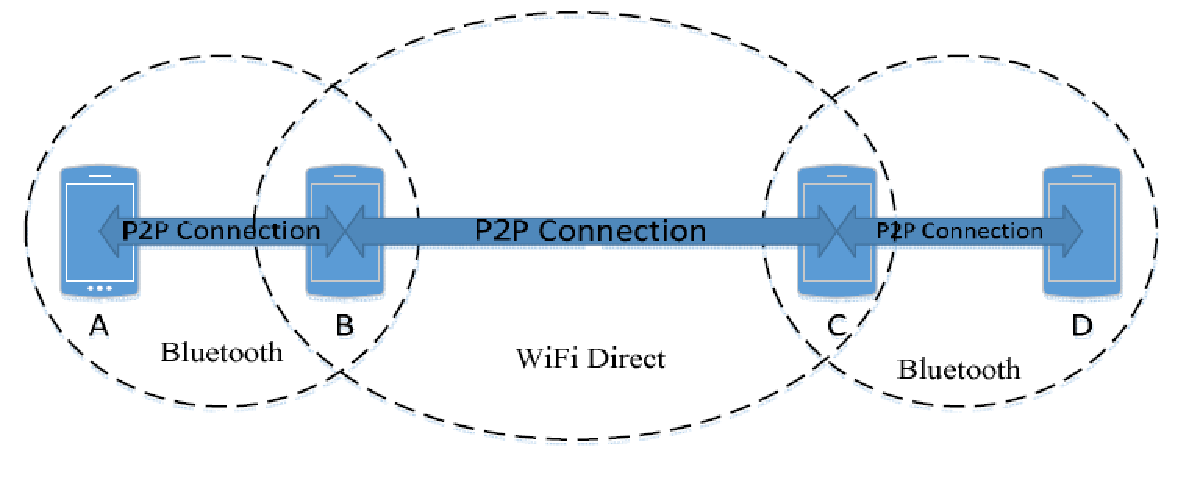
\includegraphics[width=0.8\textwidth]{images/bwmeshnet.pdf}}
	\caption{\label{fig:bwmeshnet} Overview of a preliminary network model of \textit{MultiChat}. (source: \cite{bwmesh})}
\end{figure}

The authors state that \textit{BWMesh} may be further improved in the future by:

\begin{itemize}
	\item Possibly, utilizing Bluetooth insecure communications to avoid the manual pairing of devices in the created network.
	\item Seeing Wi-Fi Direct's current Android implementation being boosted to the point where no user interaction is necessary, to transfer files between devices.
	\item Incorporating a more complex, realistic network topology. Allowing the existence of multiple multi-hop routes and destination-specific routing, for instance to allow private messaging.
\end{itemize}


